\label{subsec:exp-b2-mechanism}
The $T = 4$ matrix (\S\ref{subsec:exp-lora}) shows that $2$-bit
task-vector quantization often outperforms higher bit budgets at
worst-task NLL excess, the ``less-is-more'' dip that survives on all
four bases. An \emph{implicit-TIES} explanation is natural: $b=2$
quantization implicitly induces sparsity, playing the same role as
TIES's explicit magnitude trimming. We pre-registered two falsifiable
predictions of that hypothesis and tested both.

\paragraph{Prediction 1 (covariance with TIES): \textsc{confirmed}.}
If $b=2$ TVQ and TIES share a mechanism, their per-task excess patterns
should covary across the matrix. Pairing each (model, task, seed)
cell's $\text{dip}_t := \Delta L_t^{(b=4)} - \Delta L_t^{(b=2)}$ with
its $\text{ties\_win}_t := \Delta L_t^{(\mathrm{TA})} -
\Delta L_t^{(\mathrm{TIES})}$, the Spearman correlation across the $32$
cells is $\rho = +0.96$ (Pearson $+0.95$), above the pre-registered
$0.7$ threshold; per-model it holds $4/4$ (Llama $0.98$, Mistral
$0.95$, Qwen $0.95$, Yi $0.81$), per-task $3/4$ (GSM8K is a within-task
null where both interventions reliably help but the variation does not
covary).

\paragraph{Prediction 2 (sparsity is the shared mechanism):
\textsc{rejected}.} $b=2$ quantization does induce substantial implicit
sparsity: $50\%$ of coordinates land in the zero bucket, and
quantization error exceeds the original magnitude for $\sim 87\%$ of
coordinates. To test whether sparsity drives the dip, we built an
explicit magnitude-pruning merge (keep top-$\rho$ by $|\Delta|$, zero
the rest, sum, SVD-truncate to rank $r$) at the two densities matching
those measurements. Pruning at matched sparsity does \emph{not}
reproduce the dip; in $7$ of $8$ cells it underperforms even $b=4$
(Table~\ref{tab:e7-prune-vs-tvq}).

\begin{table}[t]
\centering
\caption{Worst-task NLL excess of explicit magnitude-pruning at the
densities matching $b=2$ TVQ's implicit sparsity, with TVQ $b=2$ and
$b=4$ for reference.}
\label{tab:e7-prune-vs-tvq}
\begin{tabular}{lrrrr}
\hline
Model & magprune $\rho=0.50$ & magprune $\rho=0.13$ & TVQ $b=2$ & TVQ $b=4$ \\
\hline
Llama-3.1-8B    & $0.225$ & $0.288$ & $0.108$ & $0.217$ \\
Mistral-7B-v0.3 & $0.155$ & $0.251$ & $0.058$ & $0.138$ \\
Qwen-2.5-7B     & $0.118$ & $0.229$ & $0.019$ & $0.105$ \\
Yi-1.5-9B       & $0.088$ & $0.151$ & $0.059$ & $0.098$ \\
\hline
\end{tabular}
\end{table}

\paragraph{Sharpened hypothesis.} The covariance with TIES is real but
not mediated by implicit sparsity. Two candidates remain open:
(i)~\emph{uniform shrinkage of large coefficients}: a min-max $b=2$
quantizer pulls the largest coefficients toward the surviving bucket
centers, and TIES's sign election under-counts sign-disagreeing
coefficients, so both compress the merged-coefficient distribution;
(ii)~\emph{per-tensor (rather than per-coordinate) calibration}:
both methods re-anchor at the tensor level, which global-density
magnitude pruning lacks. The present finding: the $b=2$ dip is real,
covaries with TIES per-task, and is \emph{not} explained by implicit
sparsity; $b=2$ and TIES behave alike because both impose tensor-level
structure on the merge, not because $b=2$ trims small coefficients.

\begin{figure}[t]
\centering
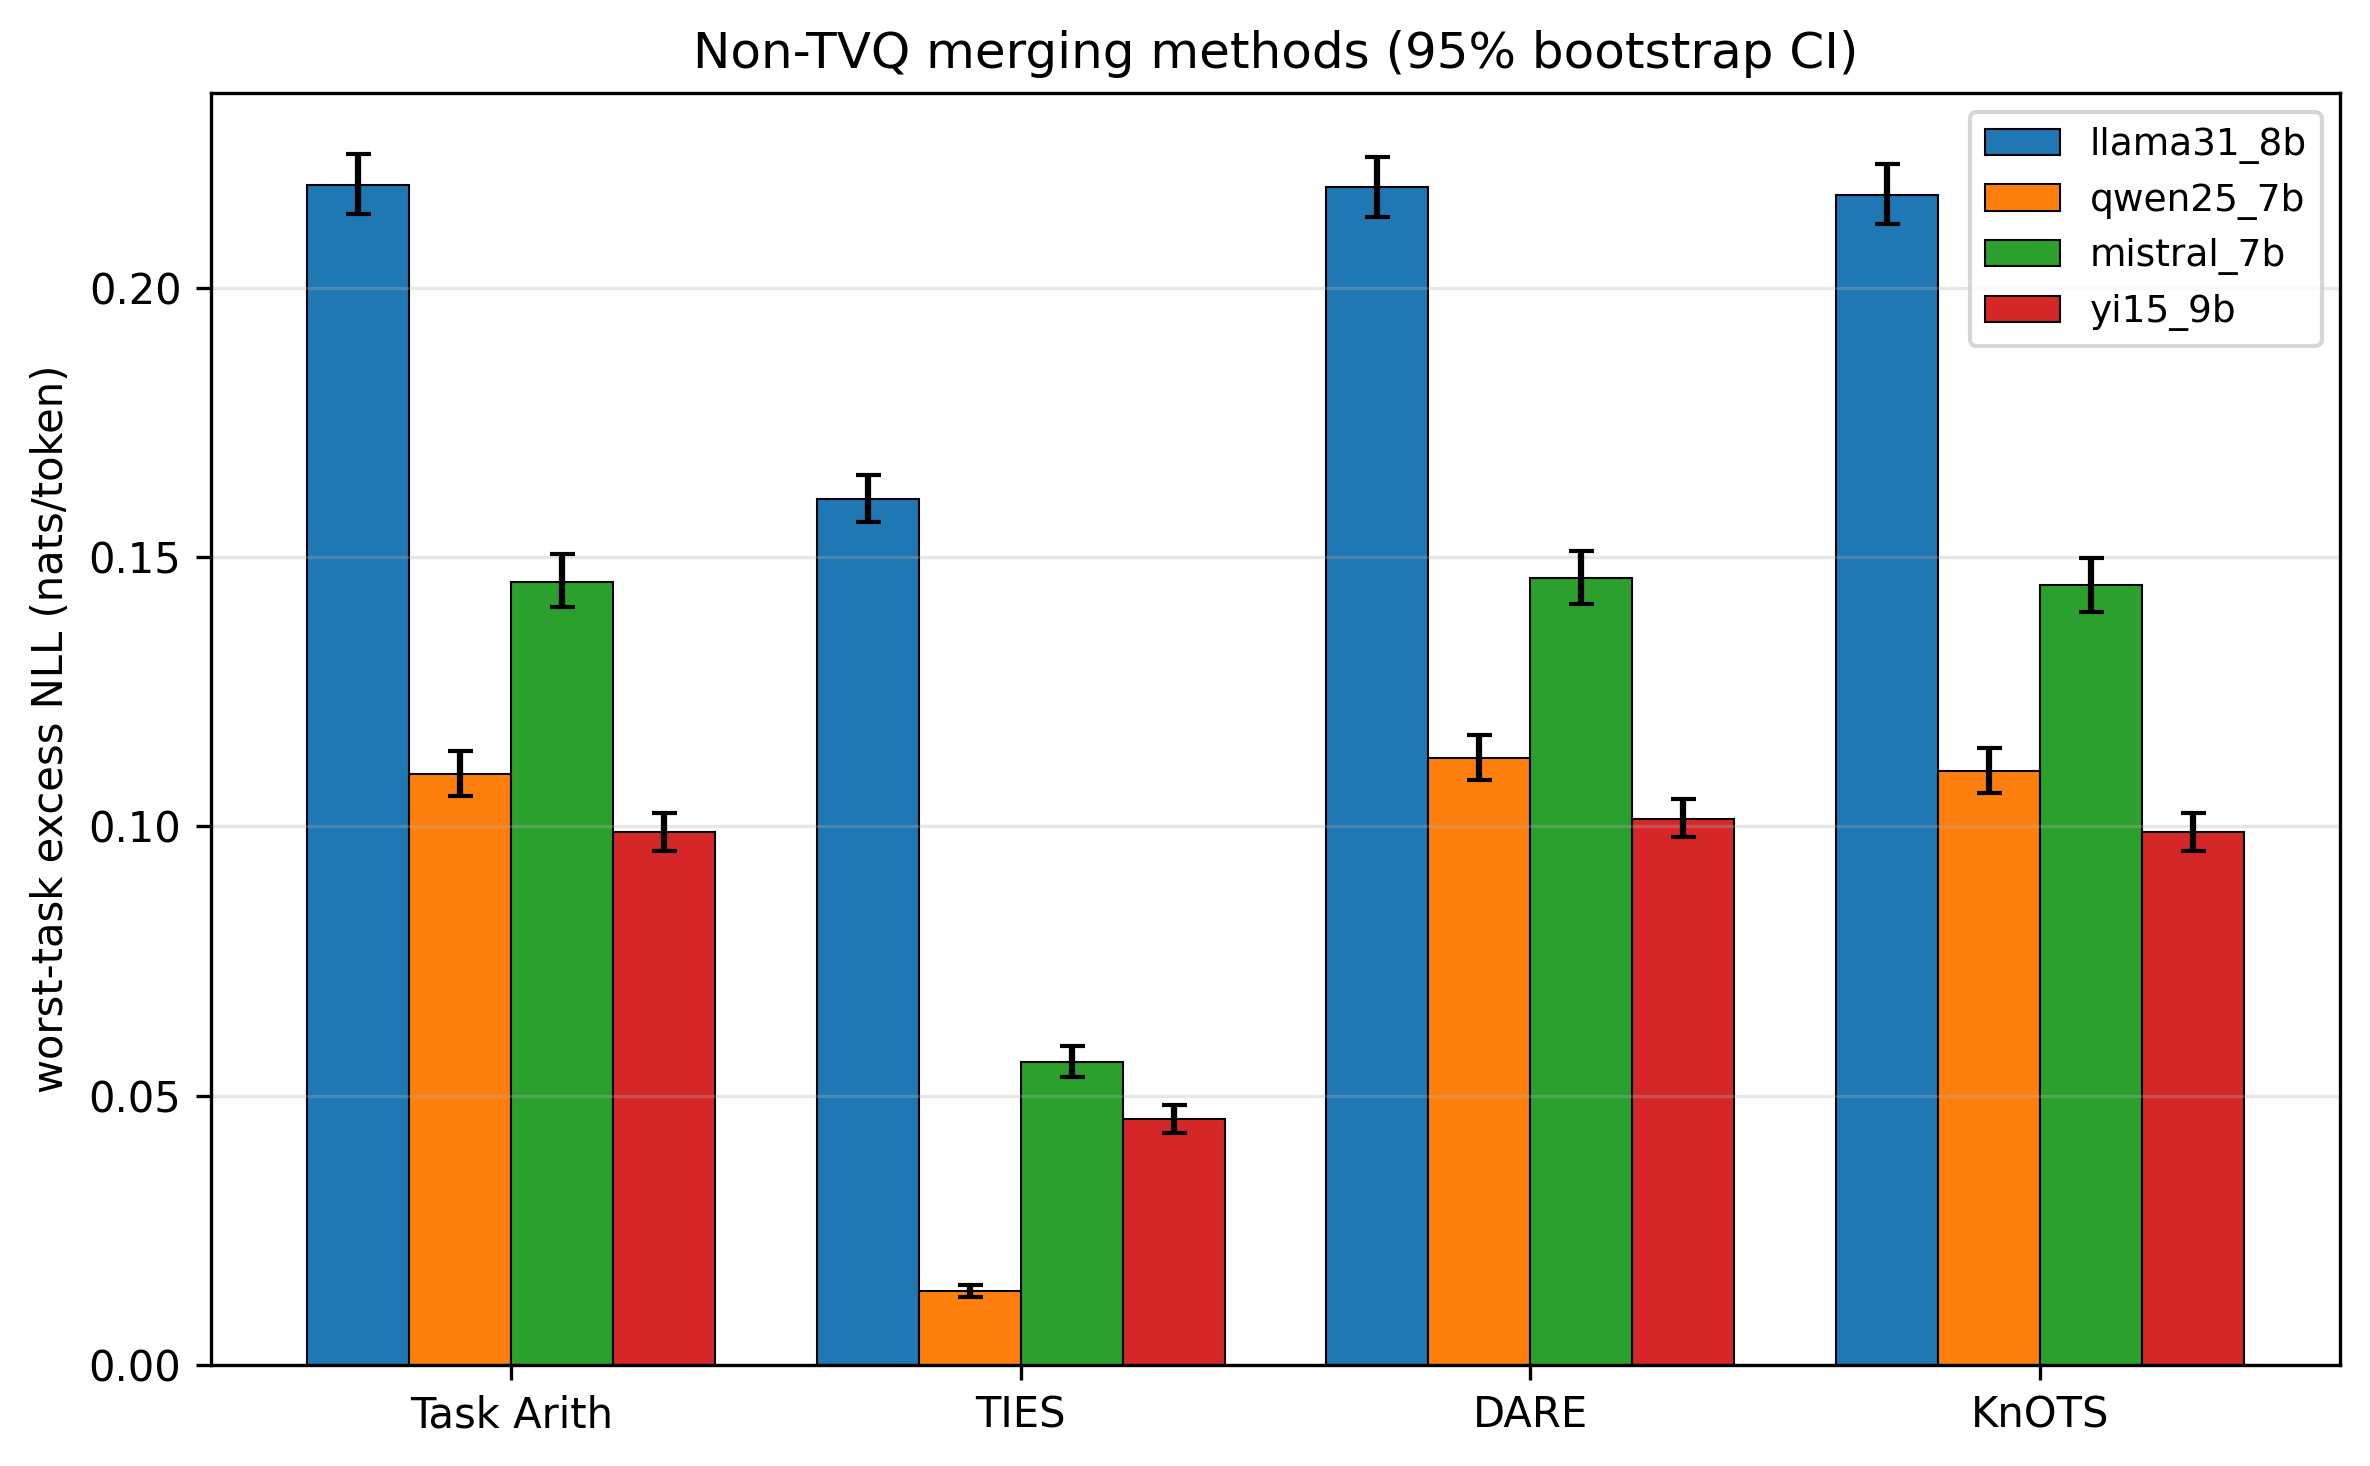
\includegraphics[width=0.7\textwidth]{figures/headline_methods_ci.png}
\caption{Non-TVQ merging methods, four architectures, $95\%$ bootstrap
CIs. Only TIES separates from the Task-Arithmetic / DARE / KnOTS
cluster.}
\label{fig:methods}
\end{figure}

\begin{figure}[t]
\centering
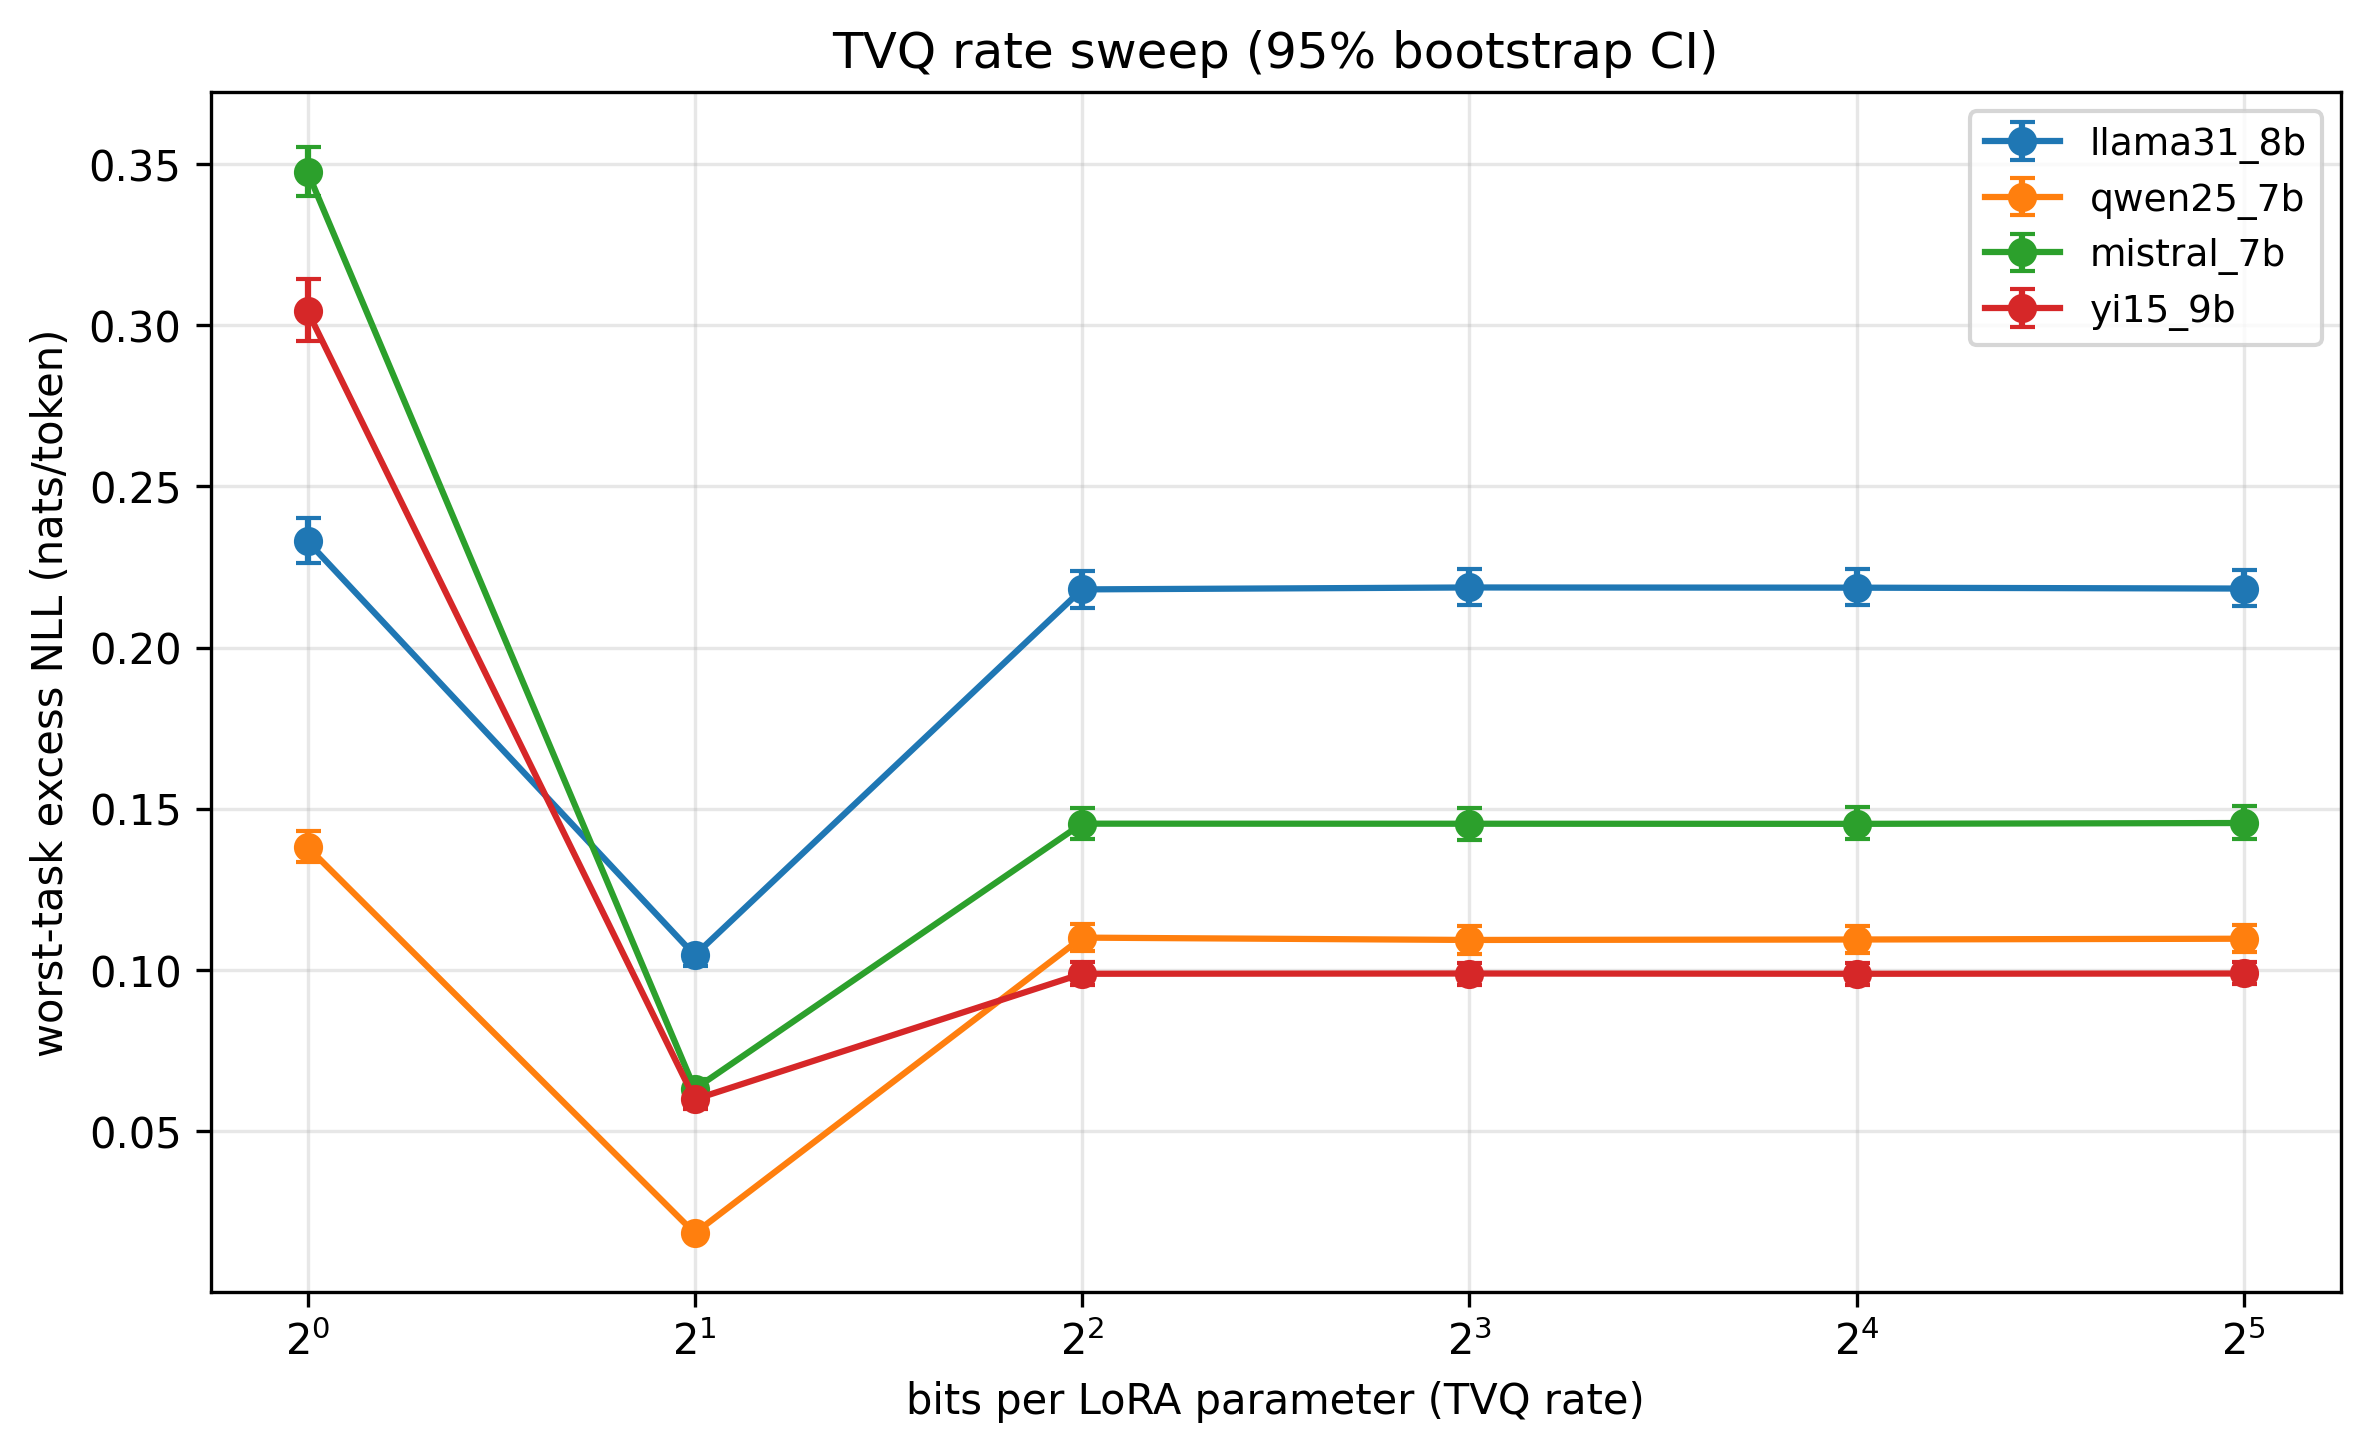
\includegraphics[width=0.7\textwidth]{figures/headline_tvq_ci.png}
\caption{TVQ rate sweep, four architectures, $95\%$ bootstrap CIs. A
universal local minimum at $b=2$ sits well below the adjacent rates on
every model; $b=1$ (too coarse) and $b\geq 4$ (too fine) regress to the
$\approx$Task-Arithmetic floor.}
\label{fig:tvq}
\end{figure}
